\documentclass[1p]{elsarticle_modified}
%\bibliographystyle{elsarticle-num}

%\usepackage[colorlinks]{hyperref}
%\usepackage{abbrmath_seonhwa} %\Abb, \Ascr, \Acal ,\Abf, \Afrak
\usepackage{amsfonts}
\usepackage{amssymb}
\usepackage{amsmath}
\usepackage{amsthm}
\usepackage{scalefnt}
\usepackage{amsbsy}
\usepackage{kotex}
\usepackage{caption}
\usepackage{subfig}
\usepackage{color}
\usepackage{graphicx}
\usepackage{xcolor} %% white, black, red, green, blue, cyan, magenta, yellow
\usepackage{float}
\usepackage{setspace}
\usepackage{hyperref}

\usepackage{tikz}
\usetikzlibrary{arrows}

\usepackage{multirow}
\usepackage{array} % fixed length table
\usepackage{hhline}

%%%%%%%%%%%%%%%%%%%%%
\makeatletter
\renewcommand*\env@matrix[1][\arraystretch]{%
	\edef\arraystretch{#1}%
	\hskip -\arraycolsep
	\let\@ifnextchar\new@ifnextchar
	\array{*\c@MaxMatrixCols c}}
\makeatother %https://tex.stackexchange.com/questions/14071/how-can-i-increase-the-line-spacing-in-a-matrix
%%%%%%%%%%%%%%%

\usepackage[normalem]{ulem}

\newcommand{\msout}[1]{\ifmmode\text{\sout{\ensuremath{#1}}}\else\sout{#1}\fi}
%SOURCE: \msout is \stkout macro in https://tex.stackexchange.com/questions/20609/strikeout-in-math-mode

\newcommand{\cancel}[1]{
	\ifmmode
	{\color{red}\msout{#1}}
	\else
	{\color{red}\sout{#1}}
	\fi
}

\newcommand{\add}[1]{
	{\color{blue}\uwave{#1}}
}

\newcommand{\replace}[2]{
	\ifmmode
	{\color{red}\msout{#1}}{\color{blue}\uwave{#2}}
	\else
	{\color{red}\sout{#1}}{\color{blue}\uwave{#2}}
	\fi
}

\newcommand{\Sol}{\mathcal{S}} %segment
\newcommand{\D}{D} %diagram
\newcommand{\A}{\mathcal{A}} %arc


%%%%%%%%%%%%%%%%%%%%%%%%%%%%%5 test

\def\sl{\operatorname{\textup{SL}}(2,\Cbb)}
\def\psl{\operatorname{\textup{PSL}}(2,\Cbb)}
\def\quan{\mkern 1mu \triangleright \mkern 1mu}

\theoremstyle{definition}
\newtheorem{thm}{Theorem}[section]
\newtheorem{prop}[thm]{Proposition}
\newtheorem{lem}[thm]{Lemma}
\newtheorem{ques}[thm]{Question}
\newtheorem{cor}[thm]{Corollary}
\newtheorem{defn}[thm]{Definition}
\newtheorem{exam}[thm]{Example}
\newtheorem{rmk}[thm]{Remark}
\newtheorem{alg}[thm]{Algorithm}

\newcommand{\I}{\sqrt{-1}}
\begin{document}

%\begin{frontmatter}
%
%\title{Boundary parabolic representations of knots up to 8 crossings}
%
%%% Group authors per affiliation:
%\author{Yunhi Cho} 
%\address{Department of Mathematics, University of Seoul, Seoul, Korea}
%\ead{yhcho@uos.ac.kr}
%
%
%\author{Seonhwa Kim} %\fnref{s_kim}}
%\address{Center for Geometry and Physics, Institute for Basic Science, Pohang, 37673, Korea}
%\ead{ryeona17@ibs.re.kr}
%
%\author{Hyuk Kim}
%\address{Department of Mathematical Sciences, Seoul National University, Seoul 08826, Korea}
%\ead{hyukkim@snu.ac.kr}
%
%\author{Seokbeom Yoon}
%\address{Department of Mathematical Sciences, Seoul National University, Seoul, 08826,  Korea}
%\ead{sbyoon15@snu.ac.kr}
%
%\begin{abstract}
%We find all boundary parabolic representation of knots up to 8 crossings.
%
%\end{abstract}
%\begin{keyword}
%    \MSC[2010] 57M25 
%\end{keyword}
%
%\end{frontmatter}

%\linenumbers
%\tableofcontents
%
\newcommand\colored[1]{\textcolor{white}{\rule[-0.35ex]{0.8em}{1.4ex}}\kern-0.8em\color{red} #1}%
%\newcommand\colored[1]{\textcolor{white}{ #1}\kern-2.17ex	\textcolor{white}{ #1}\kern-1.81ex	\textcolor{white}{ #1}\kern-2.15ex\color{red}#1	}

{\Large $\underline{11a_{74}~(K11a_{74})}$}

\setlength{\tabcolsep}{10pt}
\renewcommand{\arraystretch}{1.6}
\vspace{1cm}\begin{tabular}{m{100pt}>{\centering\arraybackslash}m{274pt}}
\multirow{5}{120pt}{
	\centering
	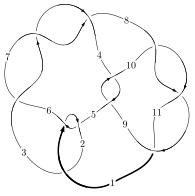
\includegraphics[width=112pt]{../../../GIT/diagram.site/Diagrams/png/323_11a_74.png}\\
\ \ \ A knot diagram\footnotemark}&
\allowdisplaybreaks
\textbf{Linearized knot diagam} \\
\cline{2-2}
 &
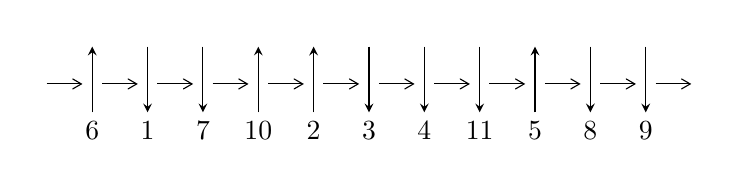
\begin{tikzpicture}[x=20pt, y=17pt]
	% nodes
	\node (C0) at (0, 0) {};
	\node (C1) at (1, 0) {};
	\node (C1U) at (1, +1) {};
	\node (C1D) at (1, -1) {6};

	\node (C2) at (2, 0) {};
	\node (C2U) at (2, +1) {};
	\node (C2D) at (2, -1) {1};

	\node (C3) at (3, 0) {};
	\node (C3U) at (3, +1) {};
	\node (C3D) at (3, -1) {7};

	\node (C4) at (4, 0) {};
	\node (C4U) at (4, +1) {};
	\node (C4D) at (4, -1) {10};

	\node (C5) at (5, 0) {};
	\node (C5U) at (5, +1) {};
	\node (C5D) at (5, -1) {2};

	\node (C6) at (6, 0) {};
	\node (C6U) at (6, +1) {};
	\node (C6D) at (6, -1) {3};

	\node (C7) at (7, 0) {};
	\node (C7U) at (7, +1) {};
	\node (C7D) at (7, -1) {4};

	\node (C8) at (8, 0) {};
	\node (C8U) at (8, +1) {};
	\node (C8D) at (8, -1) {11};

	\node (C9) at (9, 0) {};
	\node (C9U) at (9, +1) {};
	\node (C9D) at (9, -1) {5};

	\node (C10) at (10, 0) {};
	\node (C10U) at (10, +1) {};
	\node (C10D) at (10, -1) {8};

	\node (C11) at (11, 0) {};
	\node (C11U) at (11, +1) {};
	\node (C11D) at (11, -1) {9};
	\node (C12) at (12, 0) {};

	% arrows
	\draw[->,>={angle 60}]
	(C0) edge (C1) (C1) edge (C2) (C2) edge (C3) (C3) edge (C4) (C4) edge (C5) (C5) edge (C6) (C6) edge (C7) (C7) edge (C8) (C8) edge (C9) (C9) edge (C10) (C10) edge (C11) (C11) edge (C12) ;	\draw[->,>=stealth]
	(C1D) edge (C1U) (C2U) edge (C2D) (C3U) edge (C3D) (C4D) edge (C4U) (C5D) edge (C5U) (C6U) edge (C6D) (C7U) edge (C7D) (C8U) edge (C8D) (C9D) edge (C9U) (C10U) edge (C10D) (C11U) edge (C11D) ;
	\end{tikzpicture} \\
\hhline{~~} \\& 
\textbf{Solving Sequence} \\ \cline{2-2} 
 &
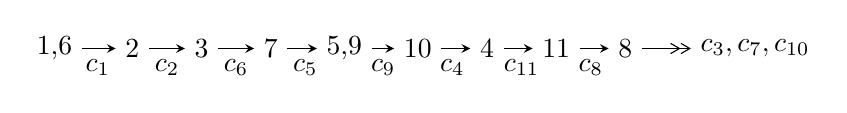
\begin{tikzpicture}[x=25pt, y=7pt]
	% node
	\node (A0) at (-1/8, 0) {1,6};
	\node (A1) at (1, 0) {2};
	\node (A2) at (2, 0) {3};
	\node (A3) at (3, 0) {7};
	\node (A4) at (65/16, 0) {5,9};
	\node (A5) at (41/8, 0) {10};
	\node (A6) at (49/8, 0) {4};
	\node (A7) at (57/8, 0) {11};
	\node (A8) at (65/8, 0) {8};
	\node (C1) at (1/2, -1) {$c_{1}$};
	\node (C2) at (3/2, -1) {$c_{2}$};
	\node (C3) at (5/2, -1) {$c_{6}$};
	\node (C4) at (7/2, -1) {$c_{5}$};
	\node (C5) at (37/8, -1) {$c_{9}$};
	\node (C6) at (45/8, -1) {$c_{4}$};
	\node (C7) at (53/8, -1) {$c_{11}$};
	\node (C8) at (61/8, -1) {$c_{8}$};
	\node (A9) at (10, 0) {$c_{3},c_{7},c_{10}$};

	% edge
	\draw[->,>=stealth]	
	(A0) edge (A1) (A1) edge (A2) (A2) edge (A3) (A3) edge (A4) (A4) edge (A5) (A5) edge (A6) (A6) edge (A7) (A7) edge (A8) ;
	\draw[->>,>={angle 60}]	
	(A8) edge (A9);
\end{tikzpicture} \\ 

\end{tabular} \\

\footnotetext{
The image of knot diagram is generated by the software ``\textbf{Draw programme}" developed by Andrew Bartholomew(\url{http://www.layer8.co.uk/maths/draw/index.htm\#Running-draw}), where we modified some parts for our purpose(\url{https://github.com/CATsTAILs/LinksPainter}).
}\phantom \\ \newline 
\centering \textbf{Ideals for irreducible components\footnotemark of $X_{\text{par}}$} 
 
\begin{align*}
I^u_{1}&=\langle 
- u^{39}- u^{38}+\cdots+b- u,\;u^{39}+u^{38}+\cdots+a+1,\;u^{41}+2 u^{40}+\cdots+u+1\rangle \\
I^u_{2}&=\langle 
b+1,\;- u^3+u^2+a- u,\;u^5- u^4+2 u^3- u^2+u-1\rangle \\
\\
\end{align*}
\raggedright * 2 irreducible components of $\dim_{\mathbb{C}}=0$, with total 46 representations.\\
\footnotetext{All coefficients of polynomials are rational numbers. But the coefficients are sometimes approximated in decimal forms when there is not enough margin.}
\newpage
\renewcommand{\arraystretch}{1}
\centering \section*{I. $I^u_{1}= \langle - u^{39}- u^{38}+\cdots+b- u,\;u^{39}+u^{38}+\cdots+a+1,\;u^{41}+2 u^{40}+\cdots+u+1 \rangle$}
\flushleft \textbf{(i) Arc colorings}\\
\begin{tabular}{m{7pt} m{180pt} m{7pt} m{180pt} }
\flushright $a_{1}=$&$\begin{pmatrix}1\\0\end{pmatrix}$ \\
\flushright $a_{6}=$&$\begin{pmatrix}0\\u\end{pmatrix}$ \\
\flushright $a_{2}=$&$\begin{pmatrix}1\\- u^2\end{pmatrix}$ \\
\flushright $a_{3}=$&$\begin{pmatrix}u^2+1\\- u^2\end{pmatrix}$ \\
\flushright $a_{7}=$&$\begin{pmatrix}- u^5-2 u^3- u\\u^5+u^3+u\end{pmatrix}$ \\
\flushright $a_{5}=$&$\begin{pmatrix}- u\\u^3+u\end{pmatrix}$ \\
\flushright $a_{9}=$&$\begin{pmatrix}- u^{39}- u^{38}+\cdots+3 u^2-1\\u^{39}+u^{38}+\cdots-2 u^2+u\end{pmatrix}$ \\
\flushright $a_{10}=$&$\begin{pmatrix}u^{38}- u^{37}+\cdots+7 u^3+2 u^2\\2 u^{39}+u^{38}+\cdots-2 u^2+2 u\end{pmatrix}$ \\
\flushright $a_{4}=$&$\begin{pmatrix}- u^8-3 u^6-3 u^4+1\\u^8+2 u^6+2 u^4\end{pmatrix}$ \\
\flushright $a_{11}=$&$\begin{pmatrix}- u^{37}- u^{36}+\cdots+2 u^2- u\\u^{39}+u^{38}+\cdots-2 u^2+2 u\end{pmatrix}$ \\
\flushright $a_{8}=$&$\begin{pmatrix}- u^{11}-4 u^9-6 u^7-2 u^5+3 u^3+2 u\\u^{11}+3 u^9+4 u^7+u^5- u^3- u\end{pmatrix}$\\ \flushright $a_{8}=$&$\begin{pmatrix}- u^{11}-4 u^9-6 u^7-2 u^5+3 u^3+2 u\\u^{11}+3 u^9+4 u^7+u^5- u^3- u\end{pmatrix}$\\&\end{tabular}
\flushleft \textbf{(ii) Obstruction class $= -1$}\\~\\
\flushleft \textbf{(iii) Cusp Shapes $= 4 u^{40}+7 u^{39}+54 u^{38}+82 u^{37}+340 u^{36}+462 u^{35}+1312 u^{34}+1616 u^{33}+3403 u^{32}+3822 u^{31}+6077 u^{30}+6214 u^{29}+7177 u^{28}+6582 u^{27}+4494 u^{26}+3388 u^{25}-1027 u^{24}-1627 u^{23}-4964 u^{22}-4460 u^{21}-4186 u^{20}-3422 u^{19}-796 u^{18}-982 u^{17}+949 u^{16}+82 u^{15}+258 u^{14}-40 u^{13}-510 u^{12}+20 u^{11}-226 u^{10}+250 u^9+184 u^8+183 u^7+146 u^6+8 u^5+26 u^4-2 u^3+6 u^2+10 u-1$}\\~\\
\newpage\renewcommand{\arraystretch}{1}
\flushleft \textbf{(iv) u-Polynomials at the component}\newline \\
\begin{tabular}{m{50pt}|m{274pt}}
Crossings & \hspace{64pt}u-Polynomials at each crossing \\
\hline $$\begin{aligned}c_{1},c_{5}\end{aligned}$$&$\begin{aligned}
&u^{41}-2 u^{40}+\cdots+u-1
\end{aligned}$\\
\hline $$\begin{aligned}c_{2}\end{aligned}$$&$\begin{aligned}
&u^{41}+24 u^{40}+\cdots+u-1
\end{aligned}$\\
\hline $$\begin{aligned}c_{3},c_{6},c_{7}\end{aligned}$$&$\begin{aligned}
&u^{41}+2 u^{40}+\cdots+21 u-9
\end{aligned}$\\
\hline $$\begin{aligned}c_{4},c_{9}\end{aligned}$$&$\begin{aligned}
&u^{41}+u^{40}+\cdots-64 u-32
\end{aligned}$\\
\hline $$\begin{aligned}c_{8},c_{10},c_{11}\end{aligned}$$&$\begin{aligned}
&u^{41}-6 u^{40}+\cdots+3 u-1
\end{aligned}$\\
\hline
\end{tabular}\\~\\
\newpage\renewcommand{\arraystretch}{1}
\flushleft \textbf{(v) Riley Polynomials at the component}\newline \\
\begin{tabular}{m{50pt}|m{274pt}}
Crossings & \hspace{64pt}Riley Polynomials at each crossing \\
\hline $$\begin{aligned}c_{1},c_{5}\end{aligned}$$&$\begin{aligned}
&y^{41}+24 y^{40}+\cdots+y-1
\end{aligned}$\\
\hline $$\begin{aligned}c_{2}\end{aligned}$$&$\begin{aligned}
&y^{41}-12 y^{40}+\cdots+33 y-1
\end{aligned}$\\
\hline $$\begin{aligned}c_{3},c_{6},c_{7}\end{aligned}$$&$\begin{aligned}
&y^{41}-48 y^{40}+\cdots+81 y-81
\end{aligned}$\\
\hline $$\begin{aligned}c_{4},c_{9}\end{aligned}$$&$\begin{aligned}
&y^{41}+33 y^{40}+\cdots+512 y-1024
\end{aligned}$\\
\hline $$\begin{aligned}c_{8},c_{10},c_{11}\end{aligned}$$&$\begin{aligned}
&y^{41}-44 y^{40}+\cdots-5 y-1
\end{aligned}$\\
\hline
\end{tabular}\\~\\
\newpage\flushleft \textbf{(vi) Complex Volumes and Cusp Shapes}
$$\begin{array}{c|c|c}  
\text{Solutions to }I^u_{1}& \I (\text{vol} + \sqrt{-1}CS) & \text{Cusp shape}\\
 \hline 
\begin{aligned}
u &= -0.364109 + 0.887001 I \\
a &= \phantom{-}0.877550 - 0.609658 I \\
b &= \phantom{-}0.140178 + 0.229591 I\end{aligned}
 & -0.38668 - 1.88770 I & -0.82834 + 4.08923 I \\ \hline\begin{aligned}
u &= -0.364109 - 0.887001 I \\
a &= \phantom{-}0.877550 + 0.609658 I \\
b &= \phantom{-}0.140178 - 0.229591 I\end{aligned}
 & -0.38668 + 1.88770 I & -0.82834 - 4.08923 I \\ \hline\begin{aligned}
u &= -0.565729 + 0.744684 I \\
a &= -1.96011 - 1.23038 I \\
b &= \phantom{-}1.43778 + 0.03286 I\end{aligned}
 & -4.81720 - 2.24797 I & -7.05405 + 3.58512 I \\ \hline\begin{aligned}
u &= -0.565729 - 0.744684 I \\
a &= -1.96011 + 1.23038 I \\
b &= \phantom{-}1.43778 - 0.03286 I\end{aligned}
 & -4.81720 + 2.24797 I & -7.05405 - 3.58512 I \\ \hline\begin{aligned}
u &= \phantom{-}0.298074 + 1.039800 I \\
a &= \phantom{-}0.514134 + 0.273626 I \\
b &= -0.700394 - 0.515888 I\end{aligned}
 & -3.51943 + 0.95935 I & -11.65925 - 0.88774 I \\ \hline\begin{aligned}
u &= \phantom{-}0.298074 - 1.039800 I \\
a &= \phantom{-}0.514134 - 0.273626 I \\
b &= -0.700394 + 0.515888 I\end{aligned}
 & -3.51943 - 0.95935 I & -11.65925 + 0.88774 I \\ \hline\begin{aligned}
u &= -0.906696 + 0.062300 I \\
a &= -0.638168 + 1.087060 I \\
b &= \phantom{-}1.59428 - 0.29257 I\end{aligned}
 & -14.7183 + 7.2472 I & -9.00971 - 3.32831 I \\ \hline\begin{aligned}
u &= -0.906696 - 0.062300 I \\
a &= -0.638168 - 1.087060 I \\
b &= \phantom{-}1.59428 + 0.29257 I\end{aligned}
 & -14.7183 - 7.2472 I & -9.00971 + 3.32831 I \\ \hline\begin{aligned}
u &= \phantom{-}0.887554\phantom{ +0.000000I} \\
a &= -0.0395218\phantom{ +0.000000I} \\
b &= -1.52039\phantom{ +0.000000I}\end{aligned}
 & -9.70106\phantom{ +0.000000I} & -8.09810\phantom{ +0.000000I} \\ \hline\begin{aligned}
u &= -0.881624 + 0.022769 I \\
a &= \phantom{-}0.255857 - 1.353200 I \\
b &= -0.605844 + 0.876406 I\end{aligned}
 & -7.47580 + 2.91735 I & -7.30362 - 2.76521 I\\
 \hline 
 \end{array}$$\newpage$$\begin{array}{c|c|c}  
\text{Solutions to }I^u_{1}& \I (\text{vol} + \sqrt{-1}CS) & \text{Cusp shape}\\
 \hline 
\begin{aligned}
u &= -0.881624 - 0.022769 I \\
a &= \phantom{-}0.255857 + 1.353200 I \\
b &= -0.605844 - 0.876406 I\end{aligned}
 & -7.47580 - 2.91735 I & -7.30362 + 2.76521 I \\ \hline\begin{aligned}
u &= \phantom{-}0.432258 + 1.033390 I \\
a &= -0.47465 - 1.53898 I \\
b &= -0.391212 + 0.669630 I\end{aligned}
 & -2.52915 + 5.16995 I & -7.30241 - 8.37437 I \\ \hline\begin{aligned}
u &= \phantom{-}0.432258 - 1.033390 I \\
a &= -0.47465 + 1.53898 I \\
b &= -0.391212 - 0.669630 I\end{aligned}
 & -2.52915 - 5.16995 I & -7.30241 + 8.37437 I \\ \hline\begin{aligned}
u &= -0.373802 + 1.057220 I \\
a &= -1.20238 + 1.81940 I \\
b &= -1.310670 - 0.105352 I\end{aligned}
 & -4.92250 - 3.20490 I & -9.59732 + 4.05642 I \\ \hline\begin{aligned}
u &= -0.373802 - 1.057220 I \\
a &= -1.20238 - 1.81940 I \\
b &= -1.310670 + 0.105352 I\end{aligned}
 & -4.92250 + 3.20490 I & -9.59732 - 4.05642 I \\ \hline\begin{aligned}
u &= \phantom{-}0.525055 + 1.060430 I \\
a &= -0.31545 + 2.34266 I \\
b &= \phantom{-}1.48731 - 0.19599 I\end{aligned}
 & -8.67231 + 8.22528 I & -10.03835 - 7.21842 I \\ \hline\begin{aligned}
u &= \phantom{-}0.525055 - 1.060430 I \\
a &= -0.31545 - 2.34266 I \\
b &= \phantom{-}1.48731 + 0.19599 I\end{aligned}
 & -8.67231 - 8.22528 I & -10.03835 + 7.21842 I \\ \hline\begin{aligned}
u &= \phantom{-}0.195299 + 1.170820 I \\
a &= \phantom{-}0.767934 + 0.191612 I \\
b &= \phantom{-}1.56724 + 0.10428 I\end{aligned}
 & -11.13990 - 1.05429 I & -13.63109 + 0.13245 I \\ \hline\begin{aligned}
u &= \phantom{-}0.195299 - 1.170820 I \\
a &= \phantom{-}0.767934 - 0.191612 I \\
b &= \phantom{-}1.56724 - 0.10428 I\end{aligned}
 & -11.13990 + 1.05429 I & -13.63109 - 0.13245 I \\ \hline\begin{aligned}
u &= \phantom{-}0.800839\phantom{ +0.000000I} \\
a &= \phantom{-}0.186265\phantom{ +0.000000I} \\
b &= \phantom{-}0.436537\phantom{ +0.000000I}\end{aligned}
 & -3.04591\phantom{ +0.000000I} & -0.386480\phantom{ +0.000000I}\\
 \hline 
 \end{array}$$\newpage$$\begin{array}{c|c|c}  
\text{Solutions to }I^u_{1}& \I (\text{vol} + \sqrt{-1}CS) & \text{Cusp shape}\\
 \hline 
\begin{aligned}
u &= \phantom{-}0.128656 + 0.767561 I \\
a &= \phantom{-}0.21319 - 1.98784 I \\
b &= -1.017510 + 0.191133 I\end{aligned}
 & -2.24222 + 0.82014 I & -9.63668 + 2.36048 I \\ \hline\begin{aligned}
u &= \phantom{-}0.128656 - 0.767561 I \\
a &= \phantom{-}0.21319 + 1.98784 I \\
b &= -1.017510 - 0.191133 I\end{aligned}
 & -2.24222 - 0.82014 I & -9.63668 - 2.36048 I \\ \hline\begin{aligned}
u &= \phantom{-}0.688250 + 0.327330 I \\
a &= -1.66239 - 0.83418 I \\
b &= \phantom{-}1.48572 + 0.13886 I\end{aligned}
 & -6.57625 - 3.60929 I & -7.29460 + 2.69532 I \\ \hline\begin{aligned}
u &= \phantom{-}0.688250 - 0.327330 I \\
a &= -1.66239 + 0.83418 I \\
b &= \phantom{-}1.48572 - 0.13886 I\end{aligned}
 & -6.57625 + 3.60929 I & -7.29460 - 2.69532 I \\ \hline\begin{aligned}
u &= -0.333948 + 0.659183 I \\
a &= \phantom{-}0.690566 + 1.131080 I \\
b &= -0.109267 - 0.349284 I\end{aligned}
 & \phantom{-}0.264887 - 1.334670 I & \phantom{-}0.48301 + 5.63905 I \\ \hline\begin{aligned}
u &= -0.333948 - 0.659183 I \\
a &= \phantom{-}0.690566 - 1.131080 I \\
b &= -0.109267 + 0.349284 I\end{aligned}
 & \phantom{-}0.264887 + 1.334670 I & \phantom{-}0.48301 - 5.63905 I \\ \hline\begin{aligned}
u &= \phantom{-}0.457167 + 1.214570 I \\
a &= \phantom{-}0.555238 + 0.444951 I \\
b &= \phantom{-}0.484933 - 0.052973 I\end{aligned}
 & -6.61640 + 4.50390 I & -3.48122 - 3.67405 I \\ \hline\begin{aligned}
u &= \phantom{-}0.457167 - 1.214570 I \\
a &= \phantom{-}0.555238 - 0.444951 I \\
b &= \phantom{-}0.484933 + 0.052973 I\end{aligned}
 & -6.61640 - 4.50390 I & -3.48122 + 3.67405 I \\ \hline\begin{aligned}
u &= -0.454729 + 1.257900 I \\
a &= \phantom{-}0.400211 - 0.118984 I \\
b &= -0.645598 + 0.885516 I\end{aligned}
 & -11.36890 - 1.81360 I & -10.77547 + 0. I\phantom{ +0.000000I} \\ \hline\begin{aligned}
u &= -0.454729 - 1.257900 I \\
a &= \phantom{-}0.400211 + 0.118984 I \\
b &= -0.645598 - 0.885516 I\end{aligned}
 & -11.36890 + 1.81360 I & -10.77547 + 0. I\phantom{ +0.000000I}\\
 \hline 
 \end{array}$$\newpage$$\begin{array}{c|c|c}  
\text{Solutions to }I^u_{1}& \I (\text{vol} + \sqrt{-1}CS) & \text{Cusp shape}\\
 \hline 
\begin{aligned}
u &= -0.478913 + 1.251130 I \\
a &= -0.91026 + 1.09596 I \\
b &= -0.586679 - 0.909041 I\end{aligned}
 & -11.19120 - 7.77933 I & -10.30522 + 0. I\phantom{ +0.000000I} \\ \hline\begin{aligned}
u &= -0.478913 - 1.251130 I \\
a &= -0.91026 - 1.09596 I \\
b &= -0.586679 + 0.909041 I\end{aligned}
 & -11.19120 + 7.77933 I & -10.30522 + 0. I\phantom{ +0.000000I} \\ \hline\begin{aligned}
u &= \phantom{-}0.468114 + 1.257970 I \\
a &= -1.26020 - 1.20638 I \\
b &= -1.53681 + 0.02313 I\end{aligned}
 & -13.5218 + 4.8223 I & -11.32712 + 0. I\phantom{ +0.000000I} \\ \hline\begin{aligned}
u &= \phantom{-}0.468114 - 1.257970 I \\
a &= -1.26020 + 1.20638 I \\
b &= -1.53681 - 0.02313 I\end{aligned}
 & -13.5218 - 4.8223 I & -11.32712 + 0. I\phantom{ +0.000000I} \\ \hline\begin{aligned}
u &= -0.433062 + 1.278700 I \\
a &= \phantom{-}0.599578 - 0.329232 I \\
b &= \phantom{-}1.61634 - 0.28380 I\end{aligned}
 & -18.8600 + 2.5415 I & -12.61033 + 0. I\phantom{ +0.000000I} \\ \hline\begin{aligned}
u &= -0.433062 - 1.278700 I \\
a &= \phantom{-}0.599578 + 0.329232 I \\
b &= \phantom{-}1.61634 + 0.28380 I\end{aligned}
 & -18.8600 - 2.5415 I & -12.61033 + 0. I\phantom{ +0.000000I} \\ \hline\begin{aligned}
u &= -0.503212 + 1.254770 I \\
a &= \phantom{-}0.78669 - 2.05025 I \\
b &= \phantom{-}1.59379 + 0.31268 I\end{aligned}
 & -18.3390 - 12.3052 I & -11.90943 + 0. I\phantom{ +0.000000I} \\ \hline\begin{aligned}
u &= -0.503212 - 1.254770 I \\
a &= \phantom{-}0.78669 + 2.05025 I \\
b &= \phantom{-}1.59379 - 0.31268 I\end{aligned}
 & -18.3390 + 12.3052 I & -11.90943 + 0. I\phantom{ +0.000000I} \\ \hline\begin{aligned}
u &= \phantom{-}0.470933 + 0.246766 I \\
a &= \phantom{-}0.87628 + 1.55909 I \\
b &= -0.369677 - 0.476409 I\end{aligned}
 & -0.44649 - 1.42241 I & -3.04926 + 5.00918 I \\ \hline\begin{aligned}
u &= \phantom{-}0.470933 - 0.246766 I \\
a &= \phantom{-}0.87628 - 1.55909 I \\
b &= -0.369677 + 0.476409 I\end{aligned}
 & -0.44649 + 1.42241 I & -3.04926 - 5.00918 I\\
 \hline 
 \end{array}$$\newpage$$\begin{array}{c|c|c}  
\text{Solutions to }I^u_{1}& \I (\text{vol} + \sqrt{-1}CS) & \text{Cusp shape}\\
 \hline 
\begin{aligned}
u &= -0.424359\phantom{ +0.000000I} \\
a &= -0.373964\phantom{ +0.000000I} \\
b &= -1.18396\phantom{ +0.000000I}\end{aligned}
 & -2.34309\phantom{ +0.000000I} & -2.85450\phantom{ +0.000000I}\\
 \hline 
 \end{array}$$\newpage\newpage\renewcommand{\arraystretch}{1}
\centering \section*{II. $I^u_{2}= \langle b+1,\;- u^3+u^2+a- u,\;u^5- u^4+2 u^3- u^2+u-1 \rangle$}
\flushleft \textbf{(i) Arc colorings}\\
\begin{tabular}{m{7pt} m{180pt} m{7pt} m{180pt} }
\flushright $a_{1}=$&$\begin{pmatrix}1\\0\end{pmatrix}$ \\
\flushright $a_{6}=$&$\begin{pmatrix}0\\u\end{pmatrix}$ \\
\flushright $a_{2}=$&$\begin{pmatrix}1\\- u^2\end{pmatrix}$ \\
\flushright $a_{3}=$&$\begin{pmatrix}u^2+1\\- u^2\end{pmatrix}$ \\
\flushright $a_{7}=$&$\begin{pmatrix}- u^4- u^2-1\\u^4- u^3+u^2+1\end{pmatrix}$ \\
\flushright $a_{5}=$&$\begin{pmatrix}- u\\u^3+u\end{pmatrix}$ \\
\flushright $a_{9}=$&$\begin{pmatrix}u^3- u^2+u\\-1\end{pmatrix}$ \\
\flushright $a_{10}=$&$\begin{pmatrix}u^3- u^2+u\\-1\end{pmatrix}$ \\
\flushright $a_{4}=$&$\begin{pmatrix}- u\\u^3+u\end{pmatrix}$ \\
\flushright $a_{11}=$&$\begin{pmatrix}u^3- u^2+u+1\\-1\end{pmatrix}$ \\
\flushright $a_{8}=$&$\begin{pmatrix}-1\\0\end{pmatrix}$\\ \flushright $a_{8}=$&$\begin{pmatrix}-1\\0\end{pmatrix}$\\&\end{tabular}
\flushleft \textbf{(ii) Obstruction class $= 1$}\\~\\
\flushleft \textbf{(iii) Cusp Shapes $= -2 u^4+7 u^3-8 u^2+6 u-12$}\\~\\
\newpage\renewcommand{\arraystretch}{1}
\flushleft \textbf{(iv) u-Polynomials at the component}\newline \\
\begin{tabular}{m{50pt}|m{274pt}}
Crossings & \hspace{64pt}u-Polynomials at each crossing \\
\hline $$\begin{aligned}c_{1}\end{aligned}$$&$\begin{aligned}
&u^5- u^4+2 u^3- u^2+u-1
\end{aligned}$\\
\hline $$\begin{aligned}c_{2}\end{aligned}$$&$\begin{aligned}
&u^5+3 u^4+4 u^3+u^2- u-1
\end{aligned}$\\
\hline $$\begin{aligned}c_{3}\end{aligned}$$&$\begin{aligned}
&u^5+u^4-2 u^3- u^2+u-1
\end{aligned}$\\
\hline $$\begin{aligned}c_{4},c_{9}\end{aligned}$$&$\begin{aligned}
&u^5
\end{aligned}$\\
\hline $$\begin{aligned}c_{5}\end{aligned}$$&$\begin{aligned}
&u^5+u^4+2 u^3+u^2+u+1
\end{aligned}$\\
\hline $$\begin{aligned}c_{6},c_{7}\end{aligned}$$&$\begin{aligned}
&u^5- u^4-2 u^3+u^2+u+1
\end{aligned}$\\
\hline $$\begin{aligned}c_{8}\end{aligned}$$&$\begin{aligned}
&(u-1)^5
\end{aligned}$\\
\hline $$\begin{aligned}c_{10},c_{11}\end{aligned}$$&$\begin{aligned}
&(u+1)^5
\end{aligned}$\\
\hline
\end{tabular}\\~\\
\newpage\renewcommand{\arraystretch}{1}
\flushleft \textbf{(v) Riley Polynomials at the component}\newline \\
\begin{tabular}{m{50pt}|m{274pt}}
Crossings & \hspace{64pt}Riley Polynomials at each crossing \\
\hline $$\begin{aligned}c_{1},c_{5}\end{aligned}$$&$\begin{aligned}
&y^5+3 y^4+4 y^3+y^2- y-1
\end{aligned}$\\
\hline $$\begin{aligned}c_{2}\end{aligned}$$&$\begin{aligned}
&y^5- y^4+8 y^3-3 y^2+3 y-1
\end{aligned}$\\
\hline $$\begin{aligned}c_{3},c_{6},c_{7}\end{aligned}$$&$\begin{aligned}
&y^5-5 y^4+8 y^3-3 y^2- y-1
\end{aligned}$\\
\hline $$\begin{aligned}c_{4},c_{9}\end{aligned}$$&$\begin{aligned}
&y^5
\end{aligned}$\\
\hline $$\begin{aligned}c_{8},c_{10},c_{11}\end{aligned}$$&$\begin{aligned}
&(y-1)^5
\end{aligned}$\\
\hline
\end{tabular}\\~\\
\newpage\flushleft \textbf{(vi) Complex Volumes and Cusp Shapes}
$$\begin{array}{c|c|c}  
\text{Solutions to }I^u_{2}& \I (\text{vol} + \sqrt{-1}CS) & \text{Cusp shape}\\
 \hline 
\begin{aligned}
u &= -0.339110 + 0.822375 I \\
a &= \phantom{-}0.871221 + 1.107660 I \\
b &= -1.00000\phantom{ +0.000000I}\end{aligned}
 & -1.97403 - 1.53058 I & -5.00899 + 6.23673 I \\ \hline\begin{aligned}
u &= -0.339110 - 0.822375 I \\
a &= \phantom{-}0.871221 - 1.107660 I \\
b &= -1.00000\phantom{ +0.000000I}\end{aligned}
 & -1.97403 + 1.53058 I & -5.00899 - 6.23673 I \\ \hline\begin{aligned}
u &= \phantom{-}0.766826\phantom{ +0.000000I} \\
a &= \phantom{-}0.629714\phantom{ +0.000000I} \\
b &= -1.00000\phantom{ +0.000000I}\end{aligned}
 & -4.04602\phantom{ +0.000000I} & -9.63840\phantom{ +0.000000I} \\ \hline\begin{aligned}
u &= \phantom{-}0.455697 + 1.200150 I \\
a &= -0.186078 - 0.874646 I \\
b &= -1.00000\phantom{ +0.000000I}\end{aligned}
 & -7.51750 + 4.40083 I & -13.17182 - 3.02310 I \\ \hline\begin{aligned}
u &= \phantom{-}0.455697 - 1.200150 I \\
a &= -0.186078 + 0.874646 I \\
b &= -1.00000\phantom{ +0.000000I}\end{aligned}
 & -7.51750 - 4.40083 I & -13.17182 + 3.02310 I\\
 \hline 
 \end{array}$$\newpage
\newpage\renewcommand{\arraystretch}{1}
\centering \section*{ III. u-Polynomials}
\begin{tabular}{m{50pt}|m{274pt}}
Crossings & \hspace{64pt}u-Polynomials at each crossing \\
\hline $$\begin{aligned}c_{1}\end{aligned}$$&$\begin{aligned}
&(u^5- u^4+2 u^3- u^2+u-1)(u^{41}-2 u^{40}+\cdots+u-1)
\end{aligned}$\\
\hline $$\begin{aligned}c_{2}\end{aligned}$$&$\begin{aligned}
&(u^5+3 u^4+4 u^3+u^2- u-1)(u^{41}+24 u^{40}+\cdots+u-1)
\end{aligned}$\\
\hline $$\begin{aligned}c_{3}\end{aligned}$$&$\begin{aligned}
&(u^5+u^4-2 u^3- u^2+u-1)(u^{41}+2 u^{40}+\cdots+21 u-9)
\end{aligned}$\\
\hline $$\begin{aligned}c_{4},c_{9}\end{aligned}$$&$\begin{aligned}
&u^5(u^{41}+u^{40}+\cdots-64 u-32)
\end{aligned}$\\
\hline $$\begin{aligned}c_{5}\end{aligned}$$&$\begin{aligned}
&(u^5+u^4+2 u^3+u^2+u+1)(u^{41}-2 u^{40}+\cdots+u-1)
\end{aligned}$\\
\hline $$\begin{aligned}c_{6},c_{7}\end{aligned}$$&$\begin{aligned}
&(u^5- u^4-2 u^3+u^2+u+1)(u^{41}+2 u^{40}+\cdots+21 u-9)
\end{aligned}$\\
\hline $$\begin{aligned}c_{8}\end{aligned}$$&$\begin{aligned}
&((u-1)^5)(u^{41}-6 u^{40}+\cdots+3 u-1)
\end{aligned}$\\
\hline $$\begin{aligned}c_{10},c_{11}\end{aligned}$$&$\begin{aligned}
&((u+1)^5)(u^{41}-6 u^{40}+\cdots+3 u-1)
\end{aligned}$\\
\hline
\end{tabular}\newpage\renewcommand{\arraystretch}{1}
\centering \section*{ IV. Riley Polynomials}
\begin{tabular}{m{50pt}|m{274pt}}
Crossings & \hspace{64pt}Riley Polynomials at each crossing \\
\hline $$\begin{aligned}c_{1},c_{5}\end{aligned}$$&$\begin{aligned}
&(y^5+3 y^4+4 y^3+y^2- y-1)(y^{41}+24 y^{40}+\cdots+y-1)
\end{aligned}$\\
\hline $$\begin{aligned}c_{2}\end{aligned}$$&$\begin{aligned}
&(y^5- y^4+8 y^3-3 y^2+3 y-1)(y^{41}-12 y^{40}+\cdots+33 y-1)
\end{aligned}$\\
\hline $$\begin{aligned}c_{3},c_{6},c_{7}\end{aligned}$$&$\begin{aligned}
&(y^5-5 y^4+8 y^3-3 y^2- y-1)(y^{41}-48 y^{40}+\cdots+81 y-81)
\end{aligned}$\\
\hline $$\begin{aligned}c_{4},c_{9}\end{aligned}$$&$\begin{aligned}
&y^5(y^{41}+33 y^{40}+\cdots+512 y-1024)
\end{aligned}$\\
\hline $$\begin{aligned}c_{8},c_{10},c_{11}\end{aligned}$$&$\begin{aligned}
&((y-1)^5)(y^{41}-44 y^{40}+\cdots-5 y-1)
\end{aligned}$\\
\hline
\end{tabular}
\vskip 2pc
\end{document}